\documentclass[times, utf8, zavrsni, numeric]{fer}
\usepackage{booktabs}
\usepackage{pdfpages}
\usepackage{graphicx}
\usepackage{float}

\begin{document}

% TODO: Navedite broj rada.
\thesisnumber{516}

% TODO: Navedite naslov rada.
\title{Detekcija zlonamjernih URL-ova}

% TODO: Navedite vaše ime i prezime.
\author{Nina Petrušić}

\maketitle

% Ispis stranice s napomenom o umetanju izvornika rada. Uklonite naredbu \izvornik ako želite izbaciti tu stranicu.
\includepdf[pages=-]{hr_0036525614_73.pdf}

% Dodavanje zahvale ili prazne stranice. Ako ne želite dodati zahvalu, naredbu ostavite radi prazne stranice.
\zahvala{}

\tableofcontents

\chapter{Uvod}
Sa sve većom popularnosti i proširenosti Interneta u svim područjima života rastu i prijetnje na Internetu. Zlonamjerni URL-ovi, odnosno zlonamjerne web stranice, jedna su od najvećih prijetnji. Navedene prijetnje najčešće se javljaju u obliku spama, phishinga, drive-by napada i social engineeringa. Spomenuti napadi uzrokuju gubitke velikih iznosa novca, ali i osobnih i povjerljivih podataka poput brojeva kreditnih kartica. \\
Tradicionalni način sprječavanja napada sa zlonamjernih stranica su crne liste (engl. \textit{blacklists}). Dokazano zlonamjerni URL-ovi stavljaju se na crne liste te se provjerava nalazi li se traženi URL na njima. Opisani način ima nekoliko velikih nedostataka - kako nove web stranice nastaju svakim danom, crne liste postaje teško za nadopunjavati te one postaju jako veliki skupovi podataka. Također, moguće je spriječiti napade s isključivo već poznatih stranica te ne omogućuju detekciju zlonamjerne stranice bez otvaranja njenog sadržaja ako se ona još ne nalazi na crnim listama. Zbog navedenih nedostataka, bio je potreban novi pristup. Metode strojnog učenja pokazale su se kao puno bolji način rješavanja problema zlonamjernih URL-ova jer rješavaju sve spomenute nedostatke crnih lista. Mnogo je metoda strojnog učenja koje se koriste za rješavanje navedenog problema, kao što su stablo odlučivanja, k-najbližih susjeda, slučajna šuma, strojni vektorski klasifikator i tako dalje. Nedostaci metoda strojnog učenja najčešće su zahtijevana količina računalnih resursa, vrijeme izvođenja te veličina skupa podataka za učenje modela.\\
U slučaju detekcije zlonamjernih URL-ova, prije učenja modela potrebno je analizirati URL te dobiti vrijednosti za odabrane parametre. Dobiveni parametri se pročišćavaju radi što točnijih rezultata te se predaju modelu za učenje. Osim pročišćavanja podataka, potrebno je i prilagoditi parametre korištene metode strojnog učenja. \\
U ovom radu korištene su i opisane dvije metode nadgledanog učenja (engl. \textit{supervised learning}) - \textbf{stablo odlučivanja} te \textbf{slučajne šume}.

\chapter{Pregled postojećih rješenja za detekciju zlonamjernih URL-ova}
Napisano je mnogo radova na temu korištenja umjetne inteligencije za rješavanje problema detekcije zlonamjernih URL-ova. U radovima se koriste različite skupine algoritama te različiti algoritmi koji pripadaju tim skupinama. \\

Istraživački rad "What's in a URL: Fast Feature Extraction and Malicious URL Detection" \cite{rad1} objašnjava korištenje algoritama mrežnog strojnog učenja (engl. \textit{online learning}) umjesto češće korištenih algoritama grupnog učenja (engl. \textit{batch  learning}) za rješavanje problema detekcije zlonamjernih URL-ova. Implementirana su i uspoređena 5 algoritma: Perceptron, Averaged Perceptron, Passive-Aggressive (i Passive-Aggressive I, Passive-Aggressive II), Confidence Weighted i Adaptive Regularization of Weights algoritmi.\\

U istraživačkom radu "Malicious URL Detection based on Machine Learning" \cite{rad2} korištena su 2 algoritma grupnog učenja (engl. \textit{batch learning}): Metoda potpornih vektora (engl. \textit{Support Vector Machine (SVM)}) i Slučajna šuma (engl. \textit{Random Forest}). Opisuje se način analize URL-ova te značajke koje su rezultat te analize.\\

Istraživački rad "Research on Malicious URL Detection Based on Random Forest"\cite{rf2} objašnjava 4 algoritma grupnog učenja (engl. \textit{batch learning}): Metoda potpornih vektora (engl. \textit{Support Vector Machine (SVM)}), K-najbližih susjeda (engl. \textit{K-Nearest Neighbors (KNN)}), Slučajna šuma (engl. \textit{Random Forest}) i Extreme Gradient Boosting (XGBOOST). Objašnjava se proces izbora parametara za svaku spomenutu metodu te se uspoređuju dobiveni rezultati algoritama.\\

Autori istraživačkog rad "Intelligent Malicious URL Detection with Feature Analysis"\cite{rad3} definiraju 41 značajku analize URL-a koje su podijeljene u 3 skupine: značajke poslužitelja, Alexa značajke (globalno, nacionalno i regionalno rankiranje web stranica) i obfuskacijske značajke. Za smanjenje kompleksnosti algoritma i vremena izvođenja korišteni su ANOVA i XGBoost algoritmi te je broj bitnih značajki sveden na 17. Korištena su i uspoređena 3 algoritma: k-najbližih susjeda, metoda potpornih vektora te XGBoost.\\

Osim tradicionalnog strojnog učenja, za rješavanje problema detekcije zlonamjernih URL-ova koriste se i ostale metode strojnog učenja i umjetne inteligencije. U istraživačkom radu "A Malicious URL Detection Method Based on CNN"\cite{rad4} koristi se metoda dubokog učenja zvana konvolucijska neuronska mreža CNN (engl. \textit{convolutional neural network}). Također, osim korištenja samo URL-a te HTML i JavaScript koda, autori koriste i dizajn i raspored elemenata na web stranici.

\chapter{Analiza URL-ova}
\section{URL}
URL, odnosno Uniform Resource Locator, poveznica je do određenog sadržaja na Internetu (HTML stranica, slika, datoteka i slično). URL se sastoji od obaveznih i opcionalnih dijelova (Slika \ref{url}). Svaki URL mora sadržavati protokol, domenu i put do datoteke.
\begin{figure}[H]
\includegraphics[width=\textwidth]{url}
\caption{Dijelovi URL-a \cite{url}}
\label{url}
\end{figure}
Najčešći protokoli su HTTP (Hypertext Transfer Protocol) i njegova sigurna verzija HTTPS (Secure HTTP), no mogući su i mailto te FTP (File Transfer Protocol). Domena se odvaja od protokola s dvotočkom i dvije kose crte "://" te je ona najčešće ime domene, ali može se koristiti i IP adresa poslužitelja. Nakon domene nalazi se put do datoteke odvojen kosom crtom. Put ne predstavlja stvarni put do datoteke na poslužitelju već je simbolički put potreban poslužitelju. Opcionalni dio s parametrima odvaja se upitnikom te se sastoji od parova ključ=vrijednost međusobno odvojenih znakom "\&". Drugi opcionalni dio URL-a je anchor koji označava dio te web stranice na koji URL vodi.

\section{Korišteni skup podataka}
Korišteni skup podataka preuzet je sa stranice Kanadskog instituta za računalnu sigurnost \cite{institut} (engl. \textit{Canadian Institute for Cybersecurity}). Skup \cite{skuppodataka} sadrži 46,800 URL-ova, od kojih je 11,500 malicioznih i 35,300 legitimnih. Sadrži 4 skupine malicioznih URL-ova: spam, phishing, malware i defacement. U ovom radu koristi se podskup podataka navedenog skupa koji sadrži 800 malicioznih i 1200 legitimnih URL-ova. Svaki URL analizira se po značajkama podijeljenim u tri skupine: \textit{leksičke značajke}, \textit{značajke sadržaja} i \textit{značajke poslužitelja}.

\section{Leksičke značajke (engl. \textit{Lexical features})}
Leksičke značajke odnose se na sam URL bez pristupa njegovom sadržaju. Zlonamjerni se URL-ovi često mogu razlikovati po duljini, entropiji, broju znamenaka u URL-u itd. Česti način oblikovanja zlonamjernog URL-a kako bi sličio legitimnom je obfuskacija. Obfuskacijom se kopira naziv legitimne stranice uz male varijacije kao što su dodavanje riječi info, support i sličnih. U ovom radu definirano je 16 leksičkih značajki.
\begin{center}
\begin{tabular}{|c|c|}
\hline
    \textbf{Značajka} & \textbf{Opis značajke} \\
    \hline \hline
    numDigits & Broj znamenki u URL-u \\
    \hline
    urlLength & Duljina URL-a \\
    \hline
    pathLength & Duljina puta do datoteke\\
    \hline
    hostLength & Duljina domene\\
    \hline
    numParameters & Broj parametara (opcionalno)\\
    \hline
    numFragments & Broj fragmenata (opcionalno)\\
    \hline
    urlProtocol & URL shema/protokol, najčešće http i https\\
    \hline
    hostIsIP &  Je li domena IP adresa poslužitelja \\
    \hline
    entropy & Entropija - količina informacija\\
    \hline
    subdirs & Broj poddirektorija u URL-u\\
    \hline
    client & Sadrži li URL riječ 'client'\\
    \hline
    login & Sadrži li URL riječ 'login'\\
    \hline
    admin & Sadrži li URL riječ 'admin'\\
    \hline
    server & Sadrži li URL riječ 'server'\\
    \hline
    periods & Broj točaka\\
    \hline
    isEncoded & Enkodiran - svaki znak zapisan koristeći '\%' i 2 heksadecimalne znamenke\\
\hline
\end{tabular}
\end{center}

\section{Značajke sadržaja (engl. \textit{Content features})}
Značajke sadržaja analiziraju preuzeti HTML kod web stranice te JavaScript skripte. Dobivamo informacije o HTML elementima, broju sakrivenih elemenata, količini JavaScript skripti na stranici, broju JavaScript eval funkcija i slično. U ovom radu korišteno je 16 značajki sadržaja.

\begin{center}
\begin{tabular}{|c|c|}
\hline
    \textbf{Značajka} & \textbf{Opis značajke} \\
    \hline \hline
    pageEntropy & Entropija - količina informacija \\
    \hline
    numOfScripts & Broj JavaScript skripti \\
    \hline
    scriptBodyRatio & Omjer količine skripti naspram tijela HTML-a\\
    \hline
    htmlLen & Duljina HTML koda\\
    \hline
    numOfHiddenTags & Broj HTML elemenata koji nisu vidljivi\\
    \hline
    numIFrames & Broj iframe elemenata\\
    \hline
    numEmbeds & Broj embed elemenata\\
    \hline
    numObjects & Broj object elemenata \\
    \hline
    numLinks & Broj poveznica\\
    \hline
    numTags & Ukupni broj HTML elemenata\\
    \hline
    numIncludedElements & Elementi koji sadrže src atribut\\
    \hline
    numWhitespaces & Broj razmaka\\
    \hline
    numEvalFunc & Broj JavaScript eval funkcija\\
    \hline
    numSentences & Broj rečenica u tekstu stranice\\
    \hline
    avgScriptLen & Prosječna duljina skripte\\
    \hline
    avgScriptEntropy & Prosječna količina informacija u skriptama\\
\hline
\end{tabular}
\end{center}

\section{Značajke poslužitelja (engl. \textit{Host features})}
Značajke poslužitelja analiziraju podatke o domeni, odnosno poslužitelju. Za analizu domene koriste se 3 python biblioteke: \textit{whois}, \textit{shodan} i \textit{waybackpy}. 
\begin{itemize}
    \item \textbf{Whois} sadrži informacije o registraciji domene, poput datuma registracije i datuma isteka registracije
    \item \textbf{Shodan} sadrži informacije o stroju na kojem je podginut poslužitelj (otvoreni portovi, operacijski sustav itd.)
    \item \textbf{The Wayback Machine} digitalna je arhiva svih stranica na Internetu te nam daje informacije o svim promjenama na zadanoj stranici tokom vremena
\end{itemize} 
U ovom radu definirano je 12 značajki poslužitelja.

\begin{center}
\begin{tabular}{|c|c|}
\hline
    \textbf{Značajka} & \textbf{Opis značajke} \\
    \hline \hline
    urlAge & Broj dana od registracije do sada \\
    \hline
    urlIntendedLifeSpan & Broj dana od registracije do isteka registracije \\
    \hline
    ttl & Vrijeme između registracije domene i prvog zapisa u wayback machine\\
    \hline
    totalUpdates & Ukupni broj promjena stranice \\
    \hline
    connectionSpeed & Brzina povezivanja na domenu \\
    \hline
    daysSinceLastSeen & Broj dana od kada je stranica zadnji put bila online \\
    \hline
    firstSeen & Datum kada je stranica prvi put zabilježena u wayback machine \\
    \hline
    urlHostIsIP & Domena je u obliku IP adrese \\
    \hline
    numOfSubdomains & Broj registriranih poddomena\\
    \hline
    urlRegCountry & Država iz koje je domena registrirana (whois) \\
    \hline
    urlHostCountry & Država u kojoj se poslužitelj nalazi (shodan) \\
    \hline
    numOpenPorts & Broj otvorenih portova (shodan) \\
\hline
\end{tabular}
\end{center}

\chapter{Algoritmi strojnog učenja}
Algoritme strojnog učenja možemo podijeliti u 3 osnovne skupine \cite{ml}:
\begin{enumerate}
    \item \textbf{nadgledano učenje} (engl. \textit{Supervised learning}) - algoritmi služe za klasificiranje podataka. Predaje im se klasificirani skup podataka za učenje te na temelju tih podataka algoritmi donose odluku. U ovu kategoriju spadaju \textit{stablo odlučivanja} i \textit{slučajne šume}.
    \item \textbf{nenadgledano učenje} (engl. \textit{Unsupervised learning}) - algoritmi ne koriste klasificirane podatke, već sami pronalaze uzorke i sličnosti u neklasificiranim podacima. Spomenuti algoritmi ne donose odluku o vrijednosti izlazne varijable, već na temelju otkrivenih uzoraka dijele podatke u skupine. 
    \item \textbf{pojačano učenje} (engl. \textit{Reinforcement learning}) - algoritmi također ne koriste klasificirane podatke. Spomenuti algoritmi uče sami sebe kroz prošle loše i dobre odluke te koriste te informacije kako bi donosili što bolje odluke.
\end{enumerate}
U ovom radu koriste se algoritmi nadgledanog učenja \textit{stablo odlučivanja} i \textit{slučajne šume}.

\section{Stablo odlučivanja (engl. \textit{Decision tree})}
Stabla odlučivanja \cite{dt} koriste se za klasifikaciju i regresiju podataka. Odluke donosi na temelju jednostavnih pravila odlučivanja koja izvodi iz podataka za učenje. Stablo ima hijerarhijsku strukturu te se sastoji od korijenskog čvora, unutarnjih čvorova, listova i grana koje međusobno povezuju čvorove (Slika \ref{Stablo}).
\begin{figure}[H]
\includegraphics[width=\textwidth]{nodes}
\caption{Hijerarhijska struktura stabla}
\label{Stablo}
\end{figure}
Svaki je unutarnji čvor jedan parametar, a grane iz njega su moguće vrijednosti tog parametra. Listovi su sve moguće vrijednosti koje možemo dobiti kao rezultat, a u slučaju detektiranja zlonamjernih URL-ova vrijednosti listova su 'legitiman' i 'zlonamjeran'. Najvažniji parametri kod stabla odlučivanja su maksimalna dubina stabla i funkcija za mjeru kvalitete grananja. Za funkciju za mjeru kvalitete grananja uzima se ili \textit{gini koeficijent} ili \textit{entropija}.
Stabla odlučivanja trebaju biti što jednostavnija, odnosno većinom nije potrebno ići u preveliku dubinu stabla, kako ne bi došlo do prenaučenosti (engl. \textit{overfitting}). Prenaučenost je rezultat prekompleksnog modela - modela koji sadrži previše nebitnih informacija ili netočne informacije. Sprječavanje prenaučenosti postiže se procesom podrezivanja (engl. \textit{pruning}) te ograničavanjem dubine stabla. Podrezivanje je proces koji odbacuje grane nastale grananjem iz značajki niske važnosti koje ne daju nove informacije i ne pomažu u donošenju odluke.\\
Stablo odlučivanja jednostavan je i intuitivan algoritam strojnog učenja koji uz dobre parametre i dobar skup podataka daje rezultate visoke točnosti. Može se koristiti i za klasifikaciju i za regresiju podataka. Nedostak ovog modela je ranije opisana prenaučenost te što mala promjena u podacima može izazvati veliku promjenu u njegovoj strukturi. Također, odlučivanje može postati previše kompleksno ako podaci sadrže velik broj značajki.

\section{Slučajne šume (engl. \textit{Random forest})}
Slučajne šume \cite{rf}\cite{rf2} su algoritam koji kombinira rezultate više stabala odlučivanja kako bi donio što točniju odluku. U slučaju klasifikacije podataka, gleda koji se od mogućih rezultata pojavljuje češće u stablima odlučivanja kao rezultat te se odlučuje za njega. Ako se koristi za regresiju, slučajna šuma računa prosjek svih rezultata dobivenih od stabala odlučivanja. Za što točnije rezultate, bitno je da je korelacija između stabala odlučivanja niska. Niska korelacija među stablima postiže se uzimanjem nasumičnog podskupa značajki (engl. \textit{the random subspace method}) za svako drvo - za razliku od običnog stabla odlučivanja koje uzima sve značajke, slučajna šuma u stablima odlučivanja uzima samo podskupe značajki.\\
Slučajna šuma ima 3 glavna parametra: broj stabala odlučivanja, maksimalna dubina svakog stabla i broj značajki u svakom stablu. Svako stablo uzima podskup podataka nazvan \textit{bootstrap sample} metodom \textit{bootstrap aggregating (bagging)} - nasumični podskup podataka za učenje s manjim promjenama u svakom stablu zbog što manje korelacije.
\begin{figure}[H]
\includegraphics[width=\textwidth]{random_forest}
\caption{Slučajna šuma}
\label{šuma}
\end{figure}
Slučajna je šuma algoritam koji daje točnije rezultate od stabla odlučivanja. Rezultati su točniji jer se koristi više stabala odlučivanja sa što manjom međusobnom korelacijom. Također, slučajna šuma ima manji rizik od prenaučenosti. Nedostaci ovog algoritma su sporija izvedba i potrebno mu je više resursa za izvođenje.

\section{Filtriranje podataka}
Kao što je spomenuto ranije, podatke je potrebno posebno pripremiti prije učenja modela. Kako ne bi došlo do overfittinga, računa se korelacija između svih parametara te se izbacuju oni parametri koji imaju visoku korelaciju (u ovoj implementaciji 0.95) s nekim drugim parametrom jer ne daju nove informacije i povećavaju kompleksnost modela. Slika \ref{Korelacija} prikazuje korelaciju parametara dobivenu za ranije definirane značajke na korištenom podskupu.
\begin{figure}[H]
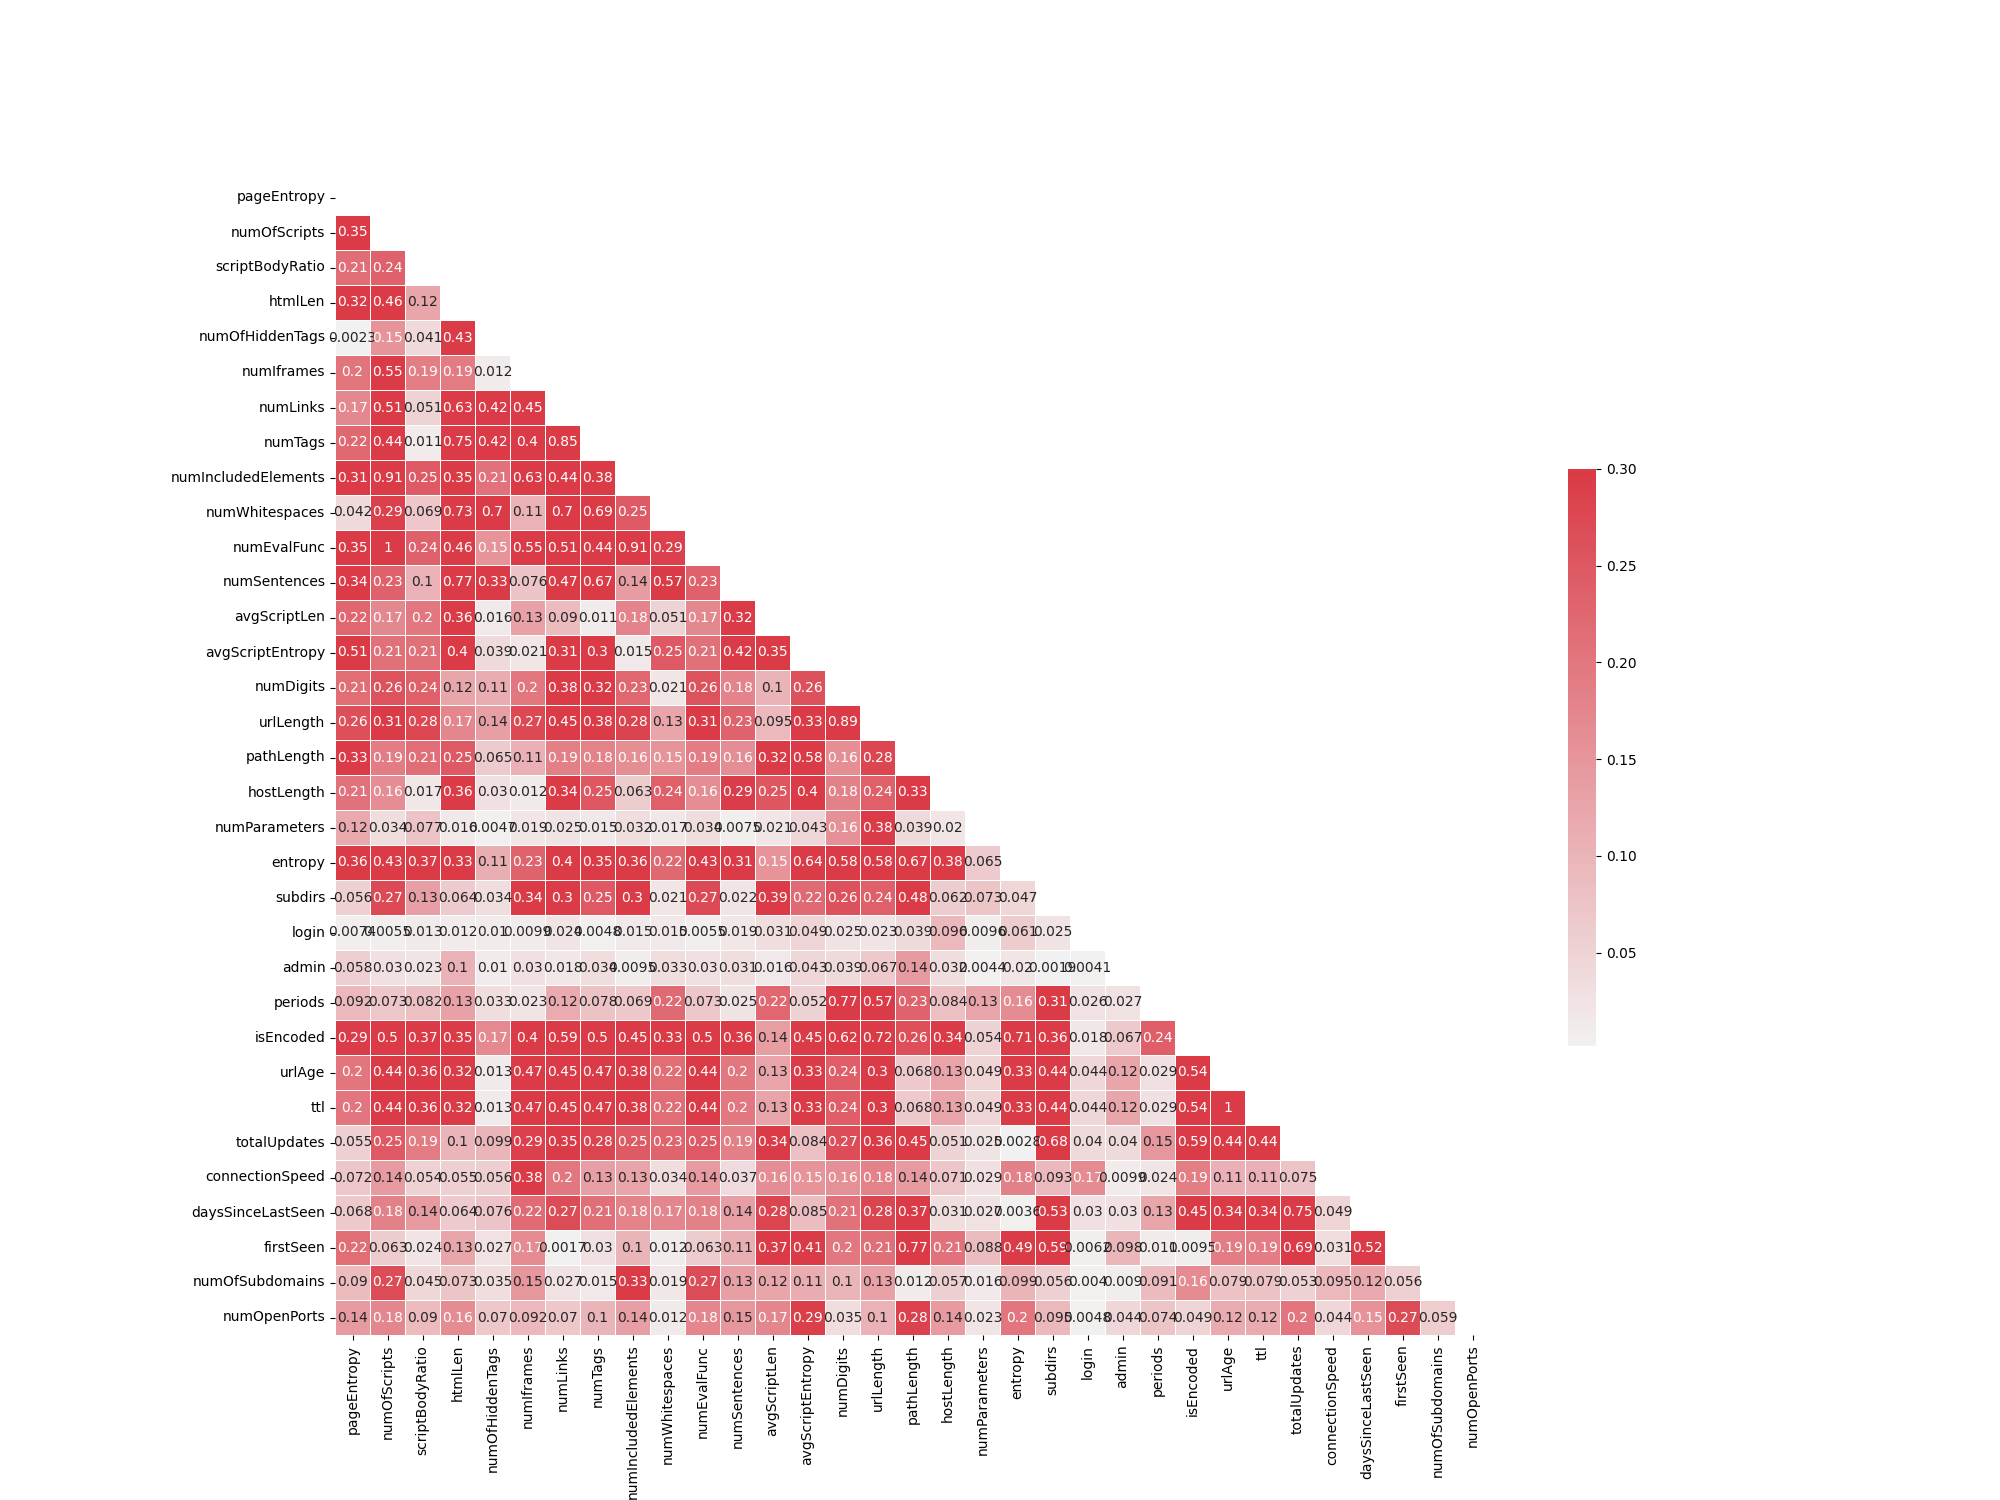
\includegraphics[width=\textwidth]{correlation}
\caption{Korelacija parametara}
\label{Korelacija}
\end{figure}

\chapter{Implementacija algoritama}
Programsko rješenje napisano je u programskom jeziku Python te koristi biblioteku \textit{scikit-learn} \cite{sl} koja sadrži potrebne algoritme strojnog učenja.
\section{Analiza skupa podataka}
U modulu \textit{data\_processing.py} obavlja se učitavanje zlonamjernih i legitimnih URL-ova iz csv datoteka te uzimanje podskupa od ranije spomenutog skupa URL-ova. Podaci su spremljeni u strukturu DataFrame iz python \textit{pandas} biblioteke. Iteriramo po skupu te se za svaki URL pozivaju funkcije iz \textit{lexicalFeatures.py, contentFeatures.py} i \textit{hostFeatures.py} koje vraćaju pojedine značajke te se rezultati spremaju u početni DataFrame. Nakon analize cijelog skupa, podaci se spremaju u datoteku \textit{ProcessedData.csv}

\subsection{Leksičke značajke}
U modulu \textit{lexicalFeatures.py} definiran je razred \texttt{lexicalFeatures}. Razred \texttt{lexicalFeatures} sadrži 16 ranije spomenutih funkcija. Slika \ref{lexicalft} prikazuje implementaciju razreda.
\begin{figure}[H]
\includegraphics[width=\textwidth]{kod_lexfeat.png}
\caption{razred lexicalFeatures}
\label{lexicalft}
\end{figure}

\subsection{Značajke sadržaja}
U modulu \textit{contentFeatures.py} definiran je razred \texttt{contentFeatures} koji sadrži 16 ranije spomenutih značajki sadržaja. Slika \ref{contentft} prikazuje isječak implementacije razreda.
\begin{figure}[H]
\includegraphics[width=\textwidth]{kod_contfeat.png}
\caption{razred contentFeatures}
\label{contentft}
\end{figure}

\subsection{Značajke poslužitelja}
U modulu \textit{hostFeatures.py} definiran je razred \texttt{hostFeatures} koji sadrži 12 ranije spomenutih značajki poslužitelja. Slika \ref{hostft} prikazuje isječak implementacije razreda.
\begin{figure}[H]
\includegraphics[width=\textwidth]{kod_hostfeat.png}
\caption{razred hostFeatures}
\label{hostft}
\end{figure}

\section{Filtriranje značajki}
Modul \textit{filter\_params.py} sastoji se od funkcije \texttt{returnFilteredData}. Funkcija računa korelaciju značajki koje su tipa int, float i bool te ju vizualizira (Slika \ref{Korelacija}) pomoću python biblioteka \textit{seaborn} i \textit{matplotlib}. U nastavku funkcije postavljamo granicu korelacije (u ovoj implementaciji postavljena je na 0.95) te iz skupa izbacujemo parametre koji su u korelaciji s drugim parametrima za vrijednost veću od te definirane granice. Nakon filtiranja, za korišteni podskup, preostali su parametri: 'pageEntropy', 'scriptBodyRatio', 'numIframes',
'numEmbeds', 'numObjects, 'numFragments', 'hostIsIP', 'client', 'server', 'login', 'admin', 'urlIntendedLifeSpan', 'totalUpdates', 'urlHostIsIP'. Slika \ref{filter} prikazuje kod funkcije \texttt{returnFilteredData}.
\begin{figure}[H]
\includegraphics[width=\textwidth]{kod_filter.png}
\caption{funkcija returnFilteredData}
\label{filter}
\end{figure}

\section{Stablo odlučivanja}
Prije izgradnje stabla potrebno je pronaći parametre s kojima stablo odlučivanja daje najtočnije rezultate. Modul \texttt{decision\_tree\_opt.py} služi za odabir najboljih parametara 'criterion' i 'max\_depth' za izgradnju stabla odlučivanja. Sastoji se od razreda \texttt{decisionTree\_opt.py} koji sadrži dvije for petlje. Jedna petlja za parametar 'criterion' (funkcija za mjeru kvalitete grananja) koristi vrijednost 'gini' te iterira po dubini stabla u rasponu 1-20. Druga petlja za parametar 'criterion' koristi vrijednost 'entropy' te također iterira po dubini stabla u rasponu 1-20. Najbolje procjene dobivene su za vrijednosti: \textit{criterion='entropy', max\_depth=5}. Također se izrađuje i sprema prikaz točnosti po isprobanim vrijednostima parametara (Slika \ref{dtcriterion}). 
\begin{figure}[H]
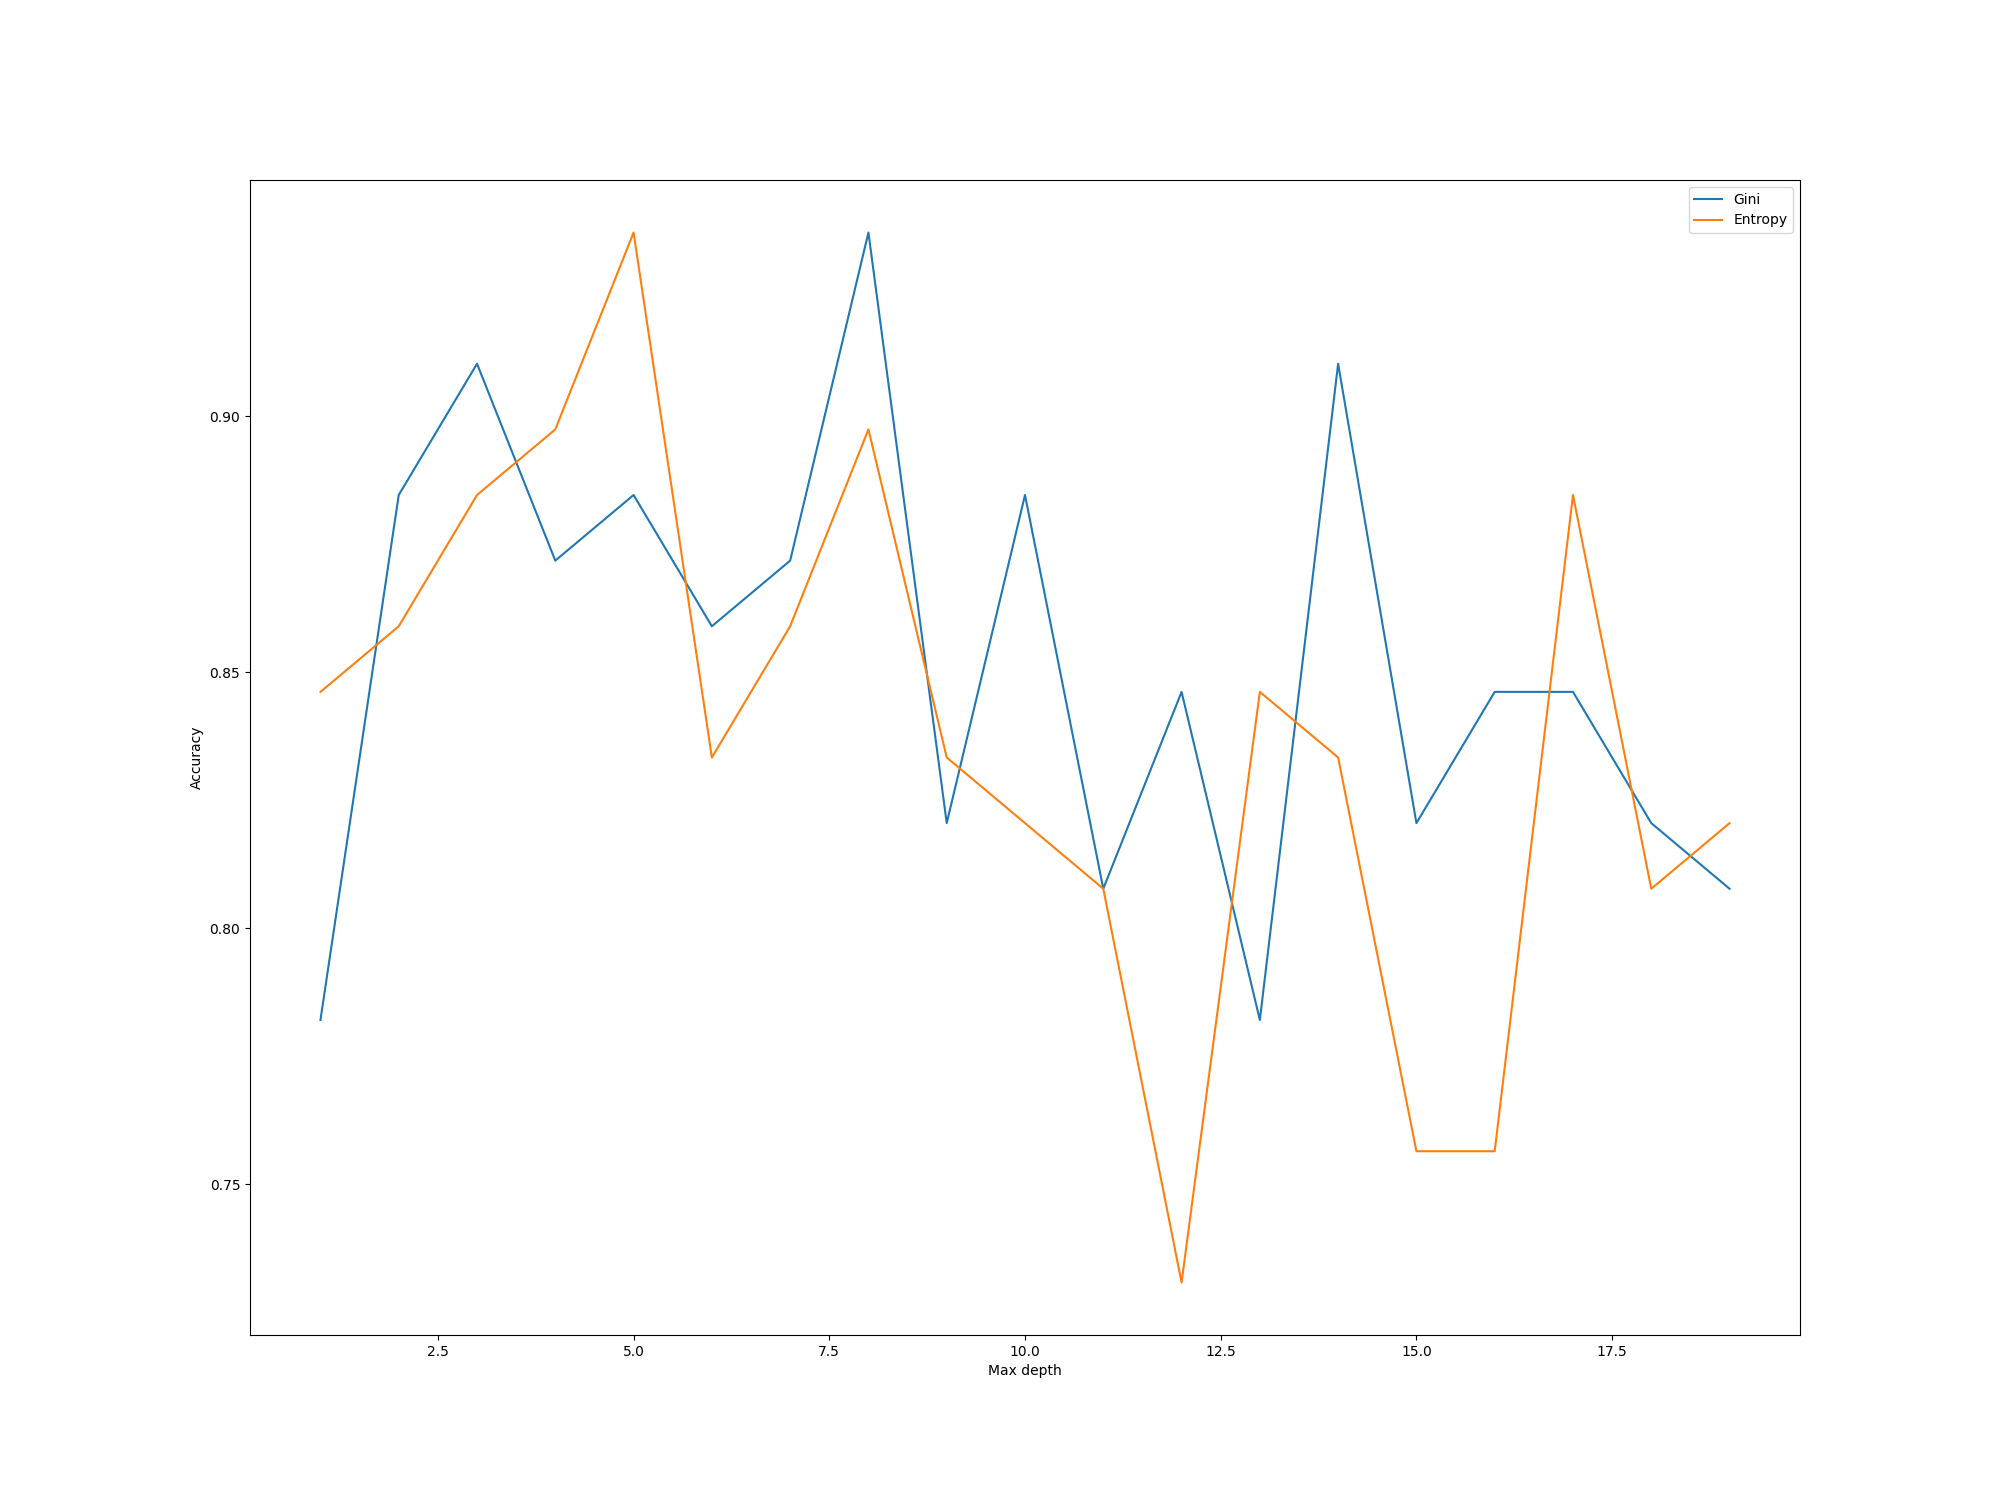
\includegraphics[width=\textwidth]{criterion.png}
\caption{Vrijednosti parametara}
\label{dtcriterion}
\end{figure}
Slika \ref{dtopt} prikazuje programski kod opisanog modula.
\begin{figure}[H]
\includegraphics[width=\textwidth]{kod_dtopt.png}
\caption{modul decision\_tree\_opt.py}
\label{dtopt}
\end{figure}

Nakon dobivenih parametara, potrebno je izgraditi stablo odlučivanja. Stablo odlučivanja implementirano je pomoću biblioteke \textit{sklearn} u modulu \texttt{decision\_tree.py}. Stablo koristi dobivene parametre \textit{criterion='entropy', max\_depth=5}. Podaci se prije učenja modela dijele na:
\begin{itemize}
    \item x\_train: 90\% podataka iz skupa, za učenje modela
    \item x\_test: klasa kojoj pojedini podatak pripada (izlazna varijabla)
    \item y\_train: 10\% podataka iz skupa, za testiranje točnosti modela
    \item y\_test: stvarni rezultati za test podatke
\end{itemize}
Nakon podjele podataka, \textit{x\_train} i \textit{y\_train} predaju se stablu koje je definirano razredom \texttt{DecisionTreeClassifier} iz biblioteke \textit{sklearn}. Sada stablu možemo predati \textit{x\_test} te rezultate usporediti sa stvarnim rezultatima \textit{y\_test}. Slika \ref{dt} prikazuje modul \texttt{decision\_tree.py}.
\begin{figure}[H]
\includegraphics[width=\textwidth]{kod_dt.png}
\caption{modul decision\_tree.py}
\label{dt}
\end{figure}

\section{Slučajna šuma}
Kao i kod stabla odlučivanja, za slučajnu je šumu potrebno pronaći parametre s kojima dobivamo najtočnije rezultate. U modulu \texttt{random\_forest\_opt.py} nalazi se klasa \texttt{randomForestOpt} koja služi za pronalaženje optimalnih parametara. Parametri za koje isprobavamo različite vrijednosti su:
\begin{itemize}
    \item \textbf{n\_estimators}: broj stabala odlučivanja u slučajnoj šumi
    \item \textbf{max\_depth}: maksimalna dubina svakog stabla odlučivanja
    \item \textbf{min\_samples\_split}: minimalni broj uzoraka potrebnih za grananje čvora
    \item \textbf{min\_samples\_leaf}: minimalni broj uzoraka koji se moraju nalaziti u listu
    \item \textbf{bootstrap}: koristi li se \textit{bootstrap aggregating}
\end{itemize}
Parametre isprobavamo pomoću razreda \texttt{RandomizedSearchCV} iz python biblioteke \textit{sklearn} koji implementira slučajno pretraživanje (engl. \textit{randomized search}). Slučajno pretraživanje uzima slučajne kombinacije zadanih parametara te ih isprobava. Najtočnije rezultate dobivamo za slijedeće vrijednosti parametara: \textit{n\_estimators=1000, min\_samples\_split=10, min\_samples\_leaf=4, max\_depth=40, bootstrap=True}. Slika \ref{rfopt} prikazuje programski kod modula \texttt{random\_forest\_opt.py}.
\begin{figure}[H]
\includegraphics[width=\textwidth]{kod_rfopt.png}
\caption{modul random\_forest\_opt.py}
\label{rfopt}
\end{figure}

Kada smo dobili optimalne parametre, izgrađujemo slučajnu šumu. Slučajna šuma implementirana je u razredu \texttt{randomForest} u modulu \texttt{random\_forest.py}. Podatke dijelimo na 'train' i 'test' podatke na isti način kao i za stablo odlučivanja, predajemo ih slučajnoj šumi koja je definirana razredom \texttt{RandomForestClassifier} iz biblioteke \textit{sklearn} te uspoređujemo rezultate. Slika \ref{rf} prikazuje programski kod modula \texttt{random\_forest.py}.
\begin{figure}[H]
\includegraphics[width=\textwidth]{kod_rf.png}
\caption{modul random\_forest.py}
\label{rf}
\end{figure}

\chapter{Rezultati}
Modul \texttt{main.py} poziva funkciju \texttt{returnFilteredData} te dobiveni skup predaje razredima \texttt{decisionTree} i \texttt{randomForest} za učenje. Navedeni razredi inicijaliziraju metode s prethodno dobivenim optimalnim parametrima i podacima te im predajemo skup od 24000 prethodno analiziranih url-ova legitimnih hrvatskih web stranica. Optimalni parametri koji se koriste su:
\begin{itemize}
    \item \textbf{Stablo odlučivanja}: critetion='entropy', max\_depth=5
    \item \textbf{Slučajna šuma}: n\_estimators=1000, min\_samples\_split=10, min\_samples\_leaf=4, max\_depth=40, bootstrap=True.
\end{itemize}
Modul \texttt{main.py} pokrenut je 5 puta zbog slučajnog načina odabira značajki i podataka za slučajnu šumu te su dobiveni sljedeći rezultati:
\begin{center}
\begin{tabular}{|c|c|c|}
\hline
    Stablo odlučivanja & Slučajna šuma & Poboljšanje\\
    \hline \hline
    90.7426\% & 92.8625\% & 2.1198\%\\
    \hline
    90.7426\% & 92.4109\% & 1.6683\%\\
    \hline
    90.7426\% & 92.6869\% & 1.9443\%\\
    \hline
    90.7426\% & 92.7120\% & 1.9694\%\\
    \hline
    90.7426\% & 92.8374\% & 2.0948\%\\
\hline
\end{tabular}
\end{center}
\begin{figure}[H]
\begin{center}
\includegraphics[width=300pt]{res.png}
\end{center}
\caption{Rezultati}
\label{res}
\end{figure}
Kako je \textit{slučajna šuma} algoritam koji koristi više \textit{stabala odlučivanja} uz ostale metode poboljšanja točnosti poput \textit{bootstrap aggregatinga}, ima očekivano bolje rezultate nego stablo odlučivanja. Zbog veće kompleksnosti, algoritam slučajna šuma zahtjeva više resursa te je njegovo izvođenje sporije nego izvođenje algoritma stabla odlučivanja.

\chapter{Zaključak}
Sigurnost na Internetu u današnjem vremenu ozbiljan je problem. Jedna sigurnosna prijetnja na webu su zlonamjerni URL-ovi koji se koriste za krađu podataka, instalaciju zloćudnih programa, novčane prevare i slično. Tradicionalne metode detektiranja zlonamjernih URL-ova poput \textit{crnih listi} postale su neefikasne. Za rješavanje problema detekcije malicioznih URL-ova sve se više koristi umjetna inteligencija, točnije strojno učenje. Ovaj pristup rješavanju spomenutog problema omogućava detekciju zlonamjernog URL-a bez potrebe da se web stranica otvori. U ovom radu opisana su i implementirana dva algoritma nadgledanog strojnog učenja: \textbf{stablo odlučivanja} koje je najpoznatiji algoritam nadgledanog učenja i algoritam koji koristi više stabala odlučivanja radi točnijih procjena - \textbf{slučajna šuma}. Rezultati su u skladu s pretpostavkama - \textit{slučajna šuma} daje točnije pretpostavke, ali zahtjeva više resursa i duže vrijeme izvođenja.

\bibliography{literatura}
\bibliographystyle{fer}

\begin{sazetak}
U radu "Detekcija zlonamjernih URL-ova" navode se problemi tradicionalnih metoda detekcije zlonamjernih URL-ova te se bavi rješavanjem problema korištenjem metoda strojnog učenja. Opisane su metode: stablo odlučivanja i slučajna šuma. Opisuje se korišteni skup podataka te način analize URL-a. Navedene metode implementirane su u programskom jeziku Python te su uspoređeni rezultati dobiveni na istom skupu podataka.

\kljucnerijeci{zlonamjerni URL, umjetna inteligencija, strojno učenje, stablo odlučivanja, slučajna šuma, Python}
\end{sazetak}

% TODO: Navedite naslov na engleskom jeziku.
\engtitle{Malicious URL detection}
\begin{abstract}
The paper "Malicious URL detection" lists problems with traditional methods for detecting malicious URLs and explains usage of machine learning methods for malicious URL detection. Methods explained and used in this paper are: decision tree and random forest. The paper describes used dataset and URL analysis. Used methods are implemented in programming language Python. Results from both methods using the described dataset are then compared.

\keywords{malicious URL, artifical intelligence, machine learning, decision tree, random forest, Python}
\end{abstract}

\end{document}
